\chapter{Introduction} \label{ch:intro}

% What is artificial intelligence & machine learning?

% Artificial intelligence (AI), and the subfield of machine learning (ML), study the processes and practicalities of enabling machines to skilfully perform intelligent tasks, without explicitly being programmed for those tasks. Recently, AI systems have neared or surpassed human performance in several tasks, such as game playing and image recognition [1], but these have typically been quite narrow and focused domains. Nonetheless, AI in its various forms is today successfully applied across a large range of domains and for challenging tasks, ranging from robotics, speech translation, image analysis and logistics to its ongoing use in designing molecules.

% Since the 1960s, medicinal chemistry has applied AI in various forms and with varying degrees of success to the design compounds. Supervised learning, where labeled training datasets are used to train models is extensively applied. An example is the quantitative structure–activity relationship (QSAR) approach, which is widely used to predict properties, such as logP, solubility and bioactivity, for given chemical structures. Conversely, unsupervised learning, which does not rely on labels, is also popular in medicinal chemistry, with examples such as hierarchical clustering, algorithms and principal components analysis being used extensively to analyze and break down large molecular libraries into smaller collections of similar compounds [2].

The discovery of new pharmaceuticals traditionally follows the design-make-test paradigm, where molecules are repeatedly proposed, synthesized, and assayed. Drug candidates are designed based on some hypothesis relating chemical structure to drug activity, which gets updated in light of new activity results. This cycle repeats as the molecular search space narrows down until a candidate molecule satisfies the necessary activity/selectivity/toxicity criteria.

\begin{figure}[!h] % !h ~ force here, t ~ top, b ~ bottom, p ~ separate page
    \centering
    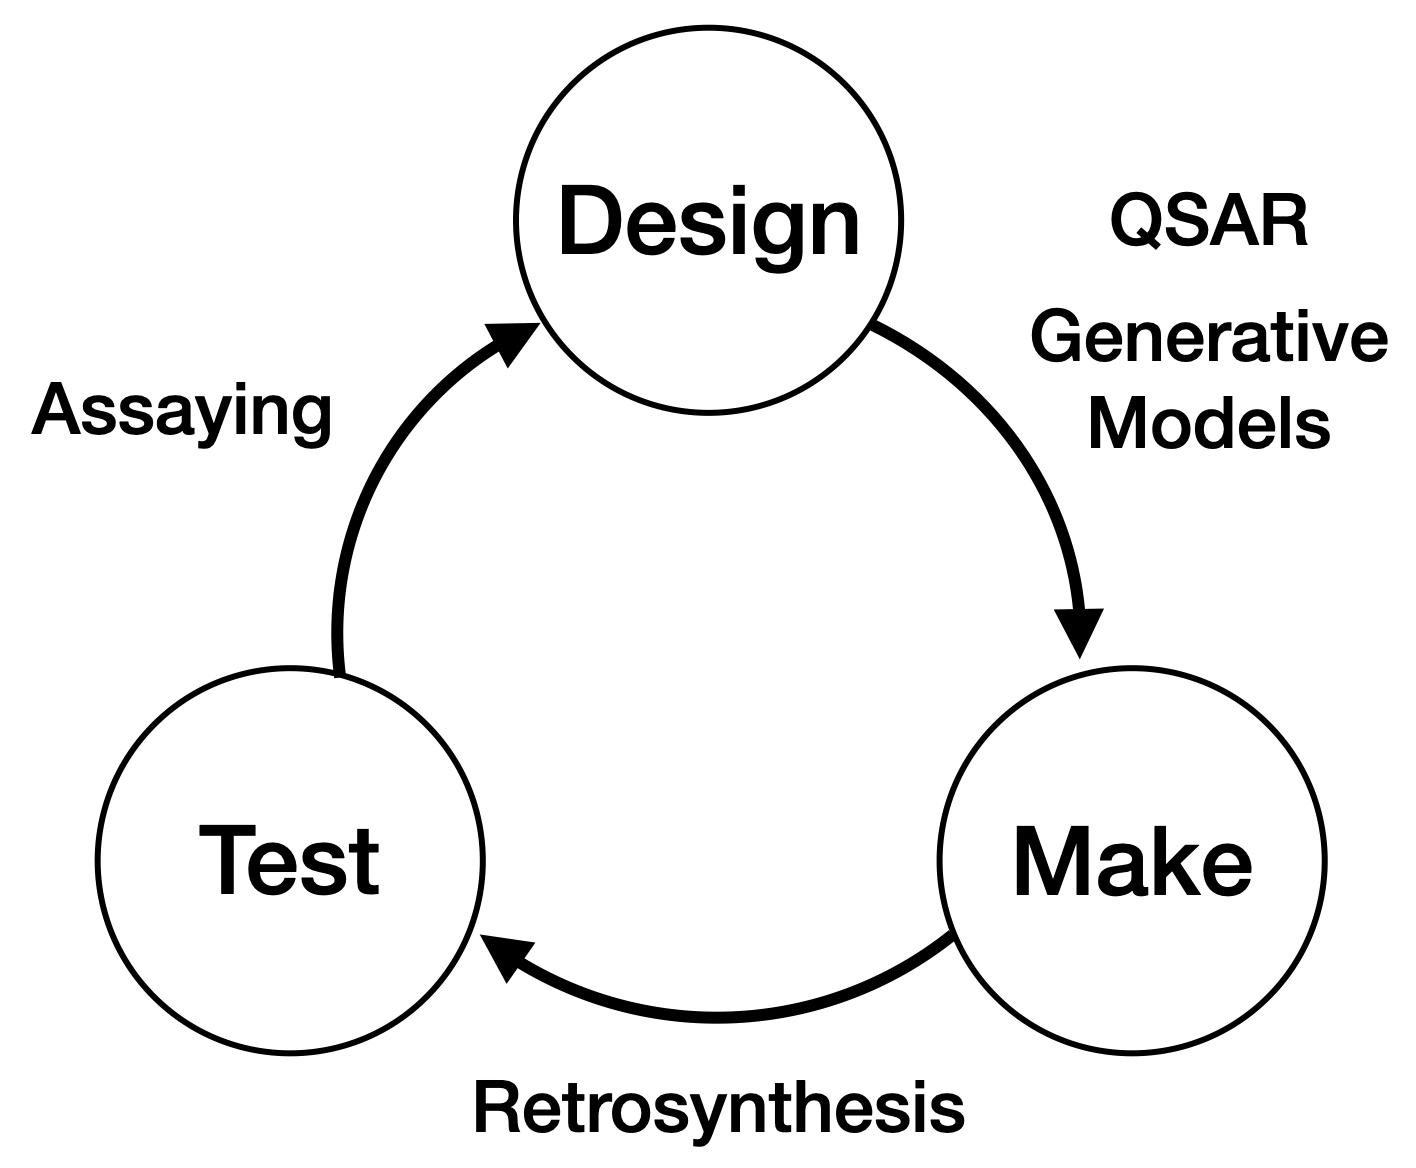
\includegraphics[width=0.5\textwidth]{Chapters/Intro/Figs/design-make-test.png}
    \caption{\label{fig:cycle} An overview of the design-make-test cycle in drug discovery.}
\end{figure}

Do a historical spiel about the application of computational methods in drug discovery, and how the field is maturing.

While computational methods have long been used in various stages of the cycle, there has been a recent surge in applying artificial intelligence to drug discovery following its success in various other fields, most notably computer vision and natural language processing. The application focus has been on `design' and `make' \cite{Coley2019AutonomousProgress}, for example in modelling quantitative structure-activity relationships (QSAR), designing generative models for proposing drug candidates, and planning retrosynthesis routes (Fig~\ref{fig:cycle}). 

% Hype versus hope: managing expectations

% The ultimate goals of applying AI and ML methods to challenges in drug discovery remain the same as they ever were: bringing the best drugs to the clinic to satisfy unmet medical need. For drug discovery and medicinal chemistry specifically, this involves tasks in identifying drug targets, identifying lead compounds, optimizing their designs against multiple property profiles of interest and identifying synthetic routes to realize the composition of matter.

% AI is often seen as a magic button that can be pressed at will to produce the perfect output, often regardless of input. Whether the AI challenge is to design the perfect image of a cat from a model trained on images of cats, a car that is able to drive itself without making a single mistake, or a drug that can be designed to treat a disease safely and efficaciously. While AI is not the answer to every challenge, it is a useful tool that if used correctly can help to augment current understanding and drive new discoveries. Within medicinal chemistry and drug discovery, the best AI is not necessarily a single AI that can autonomously design a new drug, but one or many different AIs, that enable better understanding and the design of new inputs, throughout the drug discovery process from target selection, hit identification, lead optimization to preclinical studies and clinical trials.

As the field of data-driven drug discovery matures beyond merely adapting the latest state-of-the-art machine learning (ML) methods, the present challenge is to tailor ML models specifically for the unique problems and situations faced in pharmaceutical chemistry. This thesis summarizes my efforts over the past year to play a part in this challenge with intuitions based on physical science.

\section*{Design}
The research presented in this thesis explore ways in which data-driven approaches based on machine learning can be leveraged in the design-make-test cycle of drug discovery. In each of the three steps of `design', `make', and `test' we encounter the same underlying challenge, of grappling with the practical difficulties of a drug discovery campaign where we must make full use of the limited data available.



% From the origins of atomistic theory, chemists have endeavored to predict the properties of compounds without requiring to synthesize these compounds. Alexander Crum Brown stated in 1869, that physiological response of a compound is merely a function of its chemical constitution, however defining that function remains challenging. QSARs and its relations were first proposed by Hansch and Fujita in 1962, and since this time they have remained an active area of research. The work on QSAR has led to advances into the routine of particular physicochemical property predictions, notably exemplified by ClogP, for calculating the octanol/water partition coefficient [11].

Quantitative Structure-Activity Relationship (QSAR) equations by Hansch and Frujita, emerged around the same time as machine learning and artificial intelligence, and the realted fields have shared a number of advances over the past 60 years. These QSAR equations were derived manually, orginally to be used to predicct certain molecular properties using mathematical models. In more recent decades, the processes hav emoved towards using large scale data sources and libraries of molecular descriptors to automate the generation of predictive models using more modern ML algorithms. 

The first recognised artificial intelligence application to chemistry was the Dendral system in 1965. The primary aim of the Dendral system was to study the formation of hypotheses and scientific discoveries. A path to acheiving this was the development of an expert system to analyse mass spectrometry data permitting their interpretation. Dendral is not only recognised as the first formal application of AI to chemistry, but also as the first expert system since it was capable of automating some tasks of organic chemists, such as problem solving and thereby improving decision making. 

The fields of chemistry and artificial intelligence have a long and intertwined history. indeed, chemistry led to the foundations of a number of different techniques and methods that have since found favour in artificial intelligence. From Crum Brown's definition of a predictive modelling in the mid-19th century onwards, together with the formalisation of many spects of mathematical graph theory, through early research into QSAR models and symbolic artificial intelligence in the 1960s, chemistry has been heavily involved in many advances of arificial intelligence. A number of these advances have historically been due to the primary data structure in chemical information systems being graph representations. Therefore, it logically follows that many of the algorithms developed for chemical information storage, processing and analysis have been implicitly linked with advances in graph theory.

% Since the formal advent of QSAR over 50 years ago, the numbers of modeling techniques, representations of molecules and volume of data and compute resource available have increased significantly. The advances in all of these fields mean that techniques such as deep learning that previously were not appropriate or available to these datasets can now be utilized. We now have access to large quantities of chemical structure data together with measured end points of relevance, from which it is possible to generate predictive models. However, there still remains a limited quantity of these data and even when access is available, the quality of highly variable. Here, the expectation is that more modern ML methods will be able to tackle these noisy data.

% One of the first applications of deep learning to chemical property prediction was as a result of the Merck molecular activity challenge, with multitask neural networks to predict not only one end point, but multiple end points simultaneously [12]. Deep learning chemical property prediction is now a very active area of research [13].

Short discussion on historical techniques such as molecular docking and their successes as well as limitatiions. Simulations with FEP?

In Chapter \ref{ch:fresco} we looked at how to leverage fragment-protein structures from a crystallographic fragment screen to hit discovery in the absence of any bioactivity data. Using an unsupervised learning approach, we learn the geometric distribution of pharmacophores from the fragment-protein complexes, and use these to screen potential molecules for bioactivity. We showed that this approach outperforms docking on distinguishing active compounds from inactive ones on retrospective data. Further, we prospectively found novel hits for SARS-CoV-2 Mpro and the Mac1 domain of SARS-CoV-2 non-structural protein 3 by virtually screening a library of 1B molecules.

Chapter \ref{ch:ranking} takes us to the early stages of hit-to-lead molecular optimisation where bioactivity data is limited, noisy, and dominated by inactive molecules. We overcame this challenge with a learning-to-rank framework via an ML model that predicts whether a compound is more or less active than another. This approach allowed us to make use of inactive data and threshold the bioactivity differences above measurement noise, and validation on retrospective data for SARS-CoV-2 Mpro showed that we can outperform docking on ranking ligands. Combining this model with AI-based synthesis tools, we prospectively screened a library of 8.8M molecules to arrive at a potent compound with a novel scaffold.

\section*{Make}
Likewise, another historical spiel about computer aided synthesis planning.

One of the most significant challenges in synthetic organic chemistry, let alone medicinal chemistry and drug discoveyr, is the design and planning of new chemical syntheses. Given a molecular target, what series of reactions and indeed conditions can be optimised to minimise materials, effort and time to produce the desired resutls in appropriate yield for its intended purpose in the laboratory? THese new methods take advantage of the vast repostiories of reaction data held in public databases, proprietary data held by publishers, and internal data sources at chemical companies to rapidly synthesise options of synthetic routes that have been demonstrated to be competitve with human experts. 

In recent years, AI has found significant applications to the challenge of synthetic tractability and synthesis planning. Chemical synthesis systems have later been accelerated in their potential impact by advacnes in both symbolic AI and deep learning. Indeed these recent advances have demonstrated their effectiveness through a variation of the Turing test, where expert human organic chemists were pitted against the computer software systems and able to compete well with syntehsis plans designed by the human experts. Although synthesis planning has recently been vastly improved by the advent of new algorithms, the history of AI and chemistry goes back many decades to the pioneering work of E.J. Corey. Corey developed a knowledge base of chemical reactions that could be applied in performing a retrosyntehtic analysis of target molecules, to determine a potential synthetic route. The analysis conduced would perform a logical process to predict which steps can be best conducted synthetically to achieve the target molecule. Through this process, a tree-based data structure is generated and expanded that permits optimisation of the route to suggest back to the user an optimal route.

There has been a significant amount of progress in data-driven prediction of reaction outcomes within the past decade. We can accurately predict the major products of reactions that are well-represented in our datasets as well as one can expect, given the data quality. What we can't do well is predit stereoselectivity, predict subtle cases of regioselectivity, or consider the effects of other experimental variables besides the identity of reactants and reaction conditions. As a consequence of this last point, we are, in general, unable to predict yields quantitatively unless working with datasets that hold all other vairiables constant. 

As we draw closer the theoretical worlds of design and the practical efforts of synthesis and testing of those designed compounds, so will the modern laboratory change and adapt to facilitate more close-coupled drug discovery and development and thereby enhace efficiecy and optimisation processes.

% The process of drug discovery can be summarised by the design-make-test cycle, where molecules are repeatedly proposed, synthesized, and assayed until a suitable drug candidate is found. Machine learning (ML) approaches are increasingly used to accelerate and automate all parts of this process \cite{Coley2019AutonomousOutlook, Coley2019AutonomousProgress}. The focus of the current thesis is the ``make'' part of the cycle. This is of interest because the synthesis of putative drug molecules is the most time consuming and labour intensive part of the cycle. As Blakemore et. al. \cite{Blakemore2018OrganicDiscovery} puts it ``Organic synthesis is certainly not a solved problem''. The most crucial part of the synthesis is route planning, traditionally done by expert chemists who are following the so-called disconnection approach \cite{Warren2011OrganicApproach} which is the classical framework for designing synthesis plans. Chemists usually rely on their own experience and domain knowledge, as well as databases of reactions like Reaxys \cite{ElsevierReaxysDatabase}. Nowadays, increasingly and with some success Computer Assisted Synthesis Planning tools are being used to help the chemists in designing better reaction plans \cite{Coley2018}. These tools have several advantages compared to humans: Firstly, they can quickly evaluate a very large number of possible disconnections via efficient algorithms such as Monte Carlo Tree Search \cite{Segler2018PlanningAIb}. Furthermore, by having access to exhaustive libraries of commercially available building blocks the models can disconnect into large and complex starting materials that can be readily purchased. This can reduce the number of steps and hence the risk of failure substantially.

% Planning the synthesis of novel compounds requires expertise, experience and creativity. Even though chemists can now synthesize almost everything they so desire, some compounds present themselves as tough nuts to crack. In addition, de novo design can easily suggest millions of chemical structures, only offering reasons why they should be made and not how they can be realized. Computer-aided synthesis planning (CASP) can help in both situations: by providing alternative routes or helping to prioritize compounds which can be readily synthesized.

% CASP has a long tradition, starting in the 1960s [14,15]. Ironically however, the main concept developed for CASP, working backward from the target using transformation rules and heuristics, which is now known as retrosynthetic analysis, turned out to be tremendously helpful for humans, but less so for machines.

% Recently, however, principled headway has been made. Grzybowski and coworkers reinvigorated the classic idea of heuristic-based analysis by letting experts code a large number of rules into the machine and demonstrated that the machine was able to propose tractable routes for eight medicinally relevant compounds [16].

% Going further, Segler et al. demonstrated that the computer can even learn the rules of organic chemistry autonomously from chemical reaction data without expert input [17]. Using deep neural networks they first let the machine learn to focus on the most promising rules for retroanalysis, which are then submitted to reaction prediction in combination with a modern Monte-Carlo tree search algorithm. A double-blind study, synthetic organic chemists on an average, considered the routes generated by this method to be at par with routes taken from the literature.

While AI-based synthesis tools have already shown demonstrable success in accelerating the synthesis of new molecules, they are still prone to failure and suffer from a lack of transparency in their decision making due to their black-box nature. To address this, in Chapter \ref{ch:transformer} we showcased a workflow for quantitatively interpreting a state-of-the-art deep learning model for reaction prediction. By analysing chemically selective reactions, we showed examples of correct reasoning by the model, explain counterintuitive predictions, and identify Clever Hans predictions where the correct answer is reached for the wrong reason due to dataset bias.

\section*{Test}

There are opportunities to apply machine learning methods for the interpretation of new forms of experimental data from higher-throughput experimental techniques.

In Chapter \ref{ch:testing} we explored how to accelerate testing procedures by applying machine learning on bioactivity data from nanomolar-scale high-thoughput chemistry. While this experimental technique greatly increases the number of molecules that can be tested, there is additional noise resulting from having to assay crude reaction mixtures instead of pure samples. Nevertheless, we showed that machine learning models trained on this data is able to cut through this noise and identify a false negative assay measurement, as well as prospectively screen a library of ~62K molecules to discover new SARS-CoV-2 Mpro inhibitors just as potent as those from the original assay.

% Once a feasible disconnection is found it is important to validate each step of the plan. Forward chemical reaction prediction is concerned with predicting the (major) product of an organic reaction given the reactants, reagents and preferably the conditions like solvent, temperature, concentrations etc. By having the ability to predict the product of reactions with reliable uncertainties it is possible to design clever synthesis plans where the reactions with higher uncertainty are put first. This way if a synthesis protocol fails it does so fast and cheap instead of in the later stages of the route where substantial time and cost would go to waste.

% The most successful approaches to forward reaction prediction all rely on machine learning \cite{Coley2018, Schwaller2019MolecularPrediction}. These models are trained on reaction data that is extracted from patents and publications. In these documents usually the metadata about reactions like the temperature, concentrations and solvents are found in the synthesis protocol section making it very challenging to extract this information in an automated manner. That is why these models are usually trained only on the reactants and reagents with all of the context information missing. There have been attempts at predicting the yield of the reactions as well, but they concluded that it was only possible to predict them for high throughput experiments \cite{Schwaller2020PredictionLearning} .This is largely because the yield (and sometimes even the major product) is highly dependent on the conditions making the reaction prediction task from only reactants and reagents to products ill-defined. In spite of this there are reported models achieving remarkably high near 90\% Top-1 prediction accuracy on these datasets. Therefore it is of utmost importance to validate these models to see if they are able to generalize and predict the outcome of reactions reliably or if they are learning hidden biases in the datasets which results in the seemingly strong performance.

% One way to accomplish this is with ML interpretability methods. These methods are being used increasingly in the machine learning community as a tool for evaluating model robustness \cite{Alvarez-Melis2018OnMethods}. This is especially the case in scientific applications where there is usually a large amount of prior knowledge about the systems from classical physics or chemistry. Interpretability methods can help uncover the reasoning of the models predictions in simple well understood cases where the physical or chemical cause for certain outcomes is well established. This is certainly the case for chemical reaction prediction where our understanding of mechanisms and selectivities serve as good guides for the observed reactivities. If a failure in the model's understanding is uncovered this way, a number of adversarial examples (experiments) can be designed which can than be fed back into the model as new training data. This is similar to an active learning cycle that is driven by the interpretability and human understanding of the underlying chemistry.  

% A further factor necessitating interpretability in scientific machine learning is the nature of scientific data. For example in the case of chemical reaction prediction there are a number of known or hidden biases in the commonly used datasets. One of the well-known biases is the lack of negative results, meaning that every training reaction has a good outcome. This is in contrast to reality when often if a few chemicals are mixed there is no reaction, or no well defined reaction happening. This is something the models are not able to learn from only seeing positive data.

% Last but not least, interpretability methods can be used as a tool for imputing missing metadata. In the case of reaction prediction if a model can not only predict the outcome of a reaction but it can also return a number of similar training reactions with their sources (patent ID or DOI) than these can be used by the chemist to infer what the ideal conditions (solvents, temperature etc.) are for the predicted product to be realized in the lab. We believe that this novel use of interpretability can be of great use in the reaction prediction community.

% In Chapter~\ref{chap:backgroun} an introduction to forward chemical reaction prediction is given. The most important approaches are reviewed, including \textit{ab initio} quantum mechanics based, rule based and template free machine learning methods. The Molecular Transformer \cite{Schwaller2019MolecularPrediction} is presented in detail. This is the current state-of-the-art reaction prediction model in terms of Top-1 accuracy on a standard benchmark dataset, and the interpretation of this model is the focus of the current work.

% In Chapter~\ref{chap:methods} a short review of interpretable machine learning is given. The term ``interpretability'' in the context of reaction prediction and this work is defined, and our methods for interpretation are presented in detail. This includes the Integrated Gradients method \cite{Sundararajan2017AxiomaticNetworks} which has been used for interpreting chemistry models before. We build on the work of McCloskey et. al. \cite{McCloskey2019UsingChemistry} who used IGs to understand binding prediction models on artificial datasets. We extend the method to Transformer architectures, and use it in the context of reaction predictions on real experimental data. We also present a novel method for attributing the predictions of neural network models to training data points. This is a new way of thinking about interpretation that has not been used before and that can be of great use in the reaction prediction domain.
